\documentclass[../lecture-notes.tex]{subfiles}

\begin{document}

\subsection{What the zk-SNARK is?}

Let's first discuss what zk-SNARK is.

\begin{definition}
    \textbf{zk-SNARK} – Zero-Knowledge Succinct Non-interactive ARgument of Knowledge.
\end{definition}

But what do terms like ``argument of knowledge``, ``succinct``, ``non-interactive``, and 
``zero-knowledge`` mean in this context?

\begin{itemize}
    \item \textbf{Argument of Knowledge} - a proof that the prover know data that resolves a certain
    problem, and this knowledge can be verified.
    \item \textbf{Succinct} - the proof size is relatively small and does not depend on the size of 
    the data or statement. This will be explained with examples later.
    \item \textbf{Non-interactive} - to produce the proof, the prover does not need any interaction
    with the verifier.
    \item \textbf{Zero-Knowledge} - the verifier learns nothing about the data used to produce the
    proof, despite knowing that this data resolves the given problem and that the prover possesses it.
\end{itemize}

From the above, you may also find the presence of two parties:

\begin{itemize}
    \item \textbf{Prover} - the party who knows the data that can resolve the given problem.
    \item \textbf{Verifier} - the party that wants to verify the given proof.
\end{itemize}

In essence, zk-SNARKs allow one party to prove to another that they know a value without revealing 
any information about the value itself, and do so with a proof that is both small and quick to 
verify. This makes zk-SNARKs a powerful tool for maintaining privacy and efficiency in various 
cryptographic applications.

This is pretty wide defined and maybe not so obvious if you don't have any background. Let's take a
look at the example.

\begin{example}
    Imagine you're part of a treasure hunt, and you've found a hidden treasure chest. You want to 
    prove to the treasure hunt organizer that you know where the chest is hidden without revealing
    its location. Here's how zk-SNARKs can be used in this context: \\

    \textbf{The problem}: you have found a hidden treasure chest (the secret data), and you want to
    prove to the organizer (the verifier) that you know its location without actually revealing 
    where it is. \\

    \textbf{How zk-SNARKs Help}:

    \begin{itemize}
        \item Argument of Knowledge: You create a proof that demonstrates you know the exact
        location of the treasure chest. This proof convinces the organizer that you have this 
        knowledge.
        \item Succinct: The proof you provide is very small and concise. It doesn't matter how
        large the treasure map is or how many steps it took you to find the chest, the proof remains
        compact and easy to check.
        \item Non-interactive: You don't need to have a back-and-forth conversation with the 
        organizer to create this proof. You prepare it once. The organizer can verify it without 
        needing to ask you any questions.
        \item Zero-Knowledge: The proof doesn't reveal any information about the actual location of
        the treasure chest. The organizer knows you found it, but they don't learn anything about 
        where it is hidden. \\
    \end{itemize}

    Here you can think of zk-SNARK as a golden coin from the chest where the pirates' sign is 
    engraved, so the organizer can be sure you've found the treasure.
\end{example}

But the problems that we want to solve are in a slightly different format. We can't bring a coin to
the verifier. Our goal is to prove that we've executed a specific program on a set of data that 
resolves a specific challenge or gives us a particular result.

\subsection{Arithmetic Circuits}
The cryptographic tools we've learned in the previous sections work with numbers or certain 
primitives above them, so the first question is: how do we convert a program into mathematical 
language? Additionally, we need to do this in a way that is succinct and allows us to prove 
something about it.

The \textbf{Arithmetic circuits} can help us. Similar to boolean circuits, they have gates and 
wires, but instead of the operations $\mathsf{AND}$, $\mathsf{OR}$, and $\mathsf{NOT}$, only 
multiplication and addition are allowed. Additionally, arithmetic circuits manipulate numbers 
directly, which are often elements of a prime field.

% --- Writing diagrams ---

% Define circle styles and colors
\colorlet{circle edge}{green!50!black}
\colorlet{circle area}{green!20}
\colorlet{gate edge}{blue!50!black}
\colorlet{gate area}{blue!20}

\tikzset{
    var/.style={circle, draw=circle edge, fill=circle area, thick, minimum size=1cm, text centered},
    gate/.style={circle, draw=gate edge, fill=gate area, thick, minimum size=1cm, text centered, 
        font=\itshape},
    arrow/.style={-Stealth, thick}
}

\begin{figure}[h!]
    \centering
    \vspace*{1em}
    
    \begin{minipage}{0.46\textwidth}
        \centering
        % Boolean AND and OR gates
        \begin{tabular}{cc}
            \begin{tikzpicture}
                % Nodes
                \node[var] (a) at (0, -1.5) {$a$};
                \node[var] (b) at (2, -1.5) {$b$};
                \node[gate] (and) at (1, 0) {and};
                \node[var] (c) at (1, 1.5) {$c$};

                % Arrows
                \draw[arrow] (a) -- (and);
                \draw[arrow] (b) -- (and);
                \draw[arrow, blue] (and) -- (c);
            \end{tikzpicture}
            &
            \begin{tikzpicture}
                % Nodes
                \node[var] (a) at (0, -1.5) {$a$};
                \node[var] (b) at (2, -1.5) {$b$};
                \node[gate] (or) at (1, 0) {or};
                \node[var] (c) at (1, 1.5) {$c$};

                % Arrows
                \draw[arrow] (a) -- (or);
                \draw[arrow] (b) -- (or);
                \draw[arrow, blue] (or) -- (c);
            \end{tikzpicture}
        \end{tabular}
        \caption{Boolean AND and OR Gates}
    \end{minipage}
    \hspace{0.05\textwidth} % Space between figures
    \begin{minipage}{0.46\textwidth}
        \centering
        % Addition and Multiplication gates
        \begin{tabular}{cc}
            \begin{tikzpicture}
                % Nodes
                \node[var] (a) at (0, -1.5) {$a$};
                \node[var] (b) at (2, -1.5) {$b$};
                \node[gate] (add) at (1, 0) {$+$};
                \node[var] (c) at (1, 1.5) {$c$};

                % Arrows
                \draw[arrow] (a) -- (add);
                \draw[arrow] (b) -- (add);
                \draw[arrow, blue] (add) -- (c);
            \end{tikzpicture}
            &
            \begin{tikzpicture}
                % Nodes
                \node[var] (a) at (0, -1.5) {$a$};
                \node[var] (b) at (2, -1.5) {$b$};
                \node[gate] (mul) at (1, 0) {$\times$};
                \node[var] (c) at (1, 1.5) {$c$};

                % Arrows
                \draw[arrow] (a) -- (mul);
                \draw[arrow] (b) -- (mul);
                \draw[arrow, blue] (mul) -- (c);
            \end{tikzpicture}
        \end{tabular}
        \caption{Addition and Multiplication Gates}
    \end{minipage}

    \vspace*{1em}
\end{figure}

\begin{wraptable}{r}{0.4\textwidth}
    \centering
    \vspace{-1em}
    \begin{tabular}{|c|c|c|}
        \hline
        \textbf{A} & \textbf{B} & \textbf{A AND B} \\
        \hline
        0 & 0 & 0 \\
        \hline
        0 & 1 & 0 \\
        \hline
        1 & 0 & 0 \\
        \hline
        1 & 1 & 1 \\
        \hline
    \end{tabular}
    \caption{AND Gate Truth Table}
    \label{tab:and-truth-table}
    \vspace{1em}
\end{wraptable}

% --- Finish Writing diagrams ---

The \textit{AND Gate Truth \Cref{tab:and-truth-table}} shows us the results we receive if 
particular values are supplied to the gate. The main point here is that with this table, we can 
verify the validity of logical statements. Boolean circuits receive an input vector of $\{0, 1\}$ 
and resolve to true (1) or false (0); basically, they determine if the input values satisfy the 
statement.

We can do the same with \textbf{arithmetic circuits} to verify computations without excessive 
verbosity because of binary arithmetic.

Let's take a look at some examples of programs and how can we translate them to the arithmetic
circuits.

Very simple program with a multiplication.

\begin{lstlisting}[language=C,numbers=none]
    return a * b
\end{lstlisting}

This can be represented as a circuit with only one gate:
\[ r = a \times b \]

The witness vector (solution vector) is $\mathbf{w} = (r, a, b)$, for example: $(6, 2, 3)$. We 
assume that the $a$ and $b$ are input values. 

We can think of the ``=`` in the gate as an assertion, meaning that if $a \times b$ does not equal
$r$, the assertion fails, and the input values don't resolve the circuit.

How can we translate an if statement?

\begin{lstlisting}[language=C,numbers=none]
    if (a) {
        return b * c
    } else {
        return b + c
    }
\end{lstlisting}

We can express this logic in mathematical terms as follows: "If $a$ is true, compute 
$b \times c$; otherwise, compute $b + c$." Only numerical expressions are allowed. Knowing that
$\text{true} := 1$ and $\text{false} := 0$, we can transform it as follows:
\[ r = a \times (b \times c) + (1 - a) \times (b + c) \]
Where the witness vector is: $\mathbf{w} = (r, a , b, c)$: $(6, 1, 2, 3)$, $(5, 0, 2, 3)$.\\

But, we need to verify all the intermediate steps. This can be achieved by transforming the above
equation using the simplest terms (the gates), ensuring the correctness of each step in the program: 

\begin{equation*}
    \begin{aligned}
        r_1 &= b \times c \\
        r_2 &= b + c \\
        r_3 &= 1 - a \\
        r_4 &= a \times r_1 \\
        r_5 &= r_3 \times r_2 \\
        r &= r_4 + r_5 \\
    \end{aligned}
\end{equation*}

With witness vector: $\mathbf{w} = (r, r_1, r_2, r_3, r_4, r_5, a , b, c)$: $(6, 6, 5, 0, 6, 0, 1, 2, 3)$.

\subsection{Rank-1 Constraint System}

Almost any program written in high-level programming language can be translated (compiled) into
arithmetic circuits, that are really powerfull tool. But for the ZK proof we need slightly different
format of it -- \textbf{Rank-1 Constraint System}, where the simpliest term is \textbf{constraint}. 
This offers a more flexible and general way to describe these parts.

\begin{definition}
    The \textbf{inner product} of a linear space $\mathbb{V}$ is any symmetric, linear in the first 
    argument, and positive binary function from vector space to a set of scalars. \\
    \begin{equation*}
        \langle \cdot, \cdot \rangle: \mathbb{V} \times \mathbb{V} \rightarrow \mathbb{F}
    \end{equation*}

    $\forall \mathbf{u}, \mathbf{v}, \mathbf{w} \in \mathbb{V}, \forall a \in \mathbb{F}$ the 
    following properties are satisfied:
    \begin{itemize}
        \item Symmetry: $\langle \mathbf{u}, \mathbf{v} \rangle = \langle \mathbf{v}, \mathbf{u} \rangle$
        \item Linearity in the first argument: $\langle c\mathbf{u} + \mathbf{v}, \mathbf{w} \rangle = c \langle \mathbf{u}, \mathbf{w} \rangle + \langle \mathbf{v}, \mathbf{w} \rangle$
        \item Positivity: $\langle \mathbf{u}, \mathbf{u} \rangle \geq 0$ and $\langle \mathbf{u}, \mathbf{u} \rangle = 0 \Leftrightarrow \mathbf{u} = 0$
    \end{itemize}
\end{definition}

Plenty of functions can be built that satisfy the inner product definition, we'll use the one that
is usually called \textbf{dot product}.
\begin{definition}
    Let $\mathbb{V}$ be a vector space over the field $\mathbb{F}$. The \textbf{dot product} 
    on $\mathbb{V}$ is a function:
    \begin{equation*}
        \langle \cdot, \cdot \rangle: \mathbb{V} \times \mathbb{V} \rightarrow \mathbb{F}
    \end{equation*}
    defined for $\mathbf{u}, \mathbf{v} \in \mathbb{V}$ as follows:
    \begin{equation*}
        \langle \mathbf{u}, \mathbf{v} \rangle = \sum_{i=1}^{n} u_i v_i
    \end{equation*}

    Alternatively, the dot product can also be denoted using the dot notation as:
    \begin{equation*}
        \mathbf{u} \cdot \mathbf{v}
    \end{equation*}
    That is why it's called the ``dot`` product.
\end{definition}

\begin{example}
    Let $\mathbf{u}, \mathbf{v}$ are vectors over the real number $\mathbb{R}$, where
    \begin{equation*}
        \mathbf{u} = (1, 2, 3), \quad \mathbf{v} = (2, 4, 3)
    \end{equation*}
    Then: 
    \begin{equation*}
        \langle \mathbf{u}, \mathbf{v}\rangle = \sum_{i=1}^{3}u_iv_i = 2 \cdot 1 + 2 \cdot 4 + 3 \cdot 3 = 2 + 8 + 9 = 19
    \end{equation*}
\end{example}

With knowledge of the inner product of two vectors, we can now formulate a definition of the 
constraint in the context of an R1CS.

\begin{definition}
    Each \textbf{constraint} in the Rank-1 Constraint System must be in the form:
    \begin{equation*}
        \langle \mathbf{a}, \mathbf{w}\rangle \times \langle \mathbf{b}, \mathbf{w}\rangle = \langle \mathbf{c}, \mathbf{w}\rangle
    \end{equation*}
    Where $\mathbf{w}$ is a vector containing all the \textit{input}, \textit{output}, and 
    \textit{intermediate} variables involved in the computation. The vectors $\mathbf{a}$, 
    $\mathbf{b}$, and $\mathbf{c}$ are vectors of coefficients corresponding to these variables, 
    and they define the relationship between the linear combinations of $\mathbf{w}$ on the 
    left-hand side and the right-hand side of the equation.
\end{definition}

\begin{example}
    Let's get back to our example from the previous chapter about the arithmetic circuits.
    \[ r = x_1 \times x_2 \]
    The constraint is:
    \[(a_1w_1 + a_2w_2 + a_3w_3)(b_1w_1 + b_2w_2 + b_3w_3) = c_1w_1 + c_2w_2 + c_3w_3\]
    Coefficients and witness vectors are:
    $\mathbf{w} = (r, x_1, x_2), \mathbf{a} = (0, 1, 0), \mathbf{b} = (0, 0, 1), \mathbf{c} = (1, 0, 0)$. Therefore:
    \[ (0w_1 + 1w_2 + 0w_3)(0w_1 + 0w_2 + 1w_3) = (1w_1 + 0w_2 + 0w_3) \]
    \[ w_2 \times w_3 = w_1 \]
    \[ x_1 \times x_2 = r \]
\end{example}

The interesting thing is where to take a constants from. The solution is straightforward: by placing
1 in the witness vector, so we can obtain any desired value by multiplying it by an appropriate 
coefficient.

\begin{example}
    And a more complex example. Remember that we want to verify each computational step.

    \begin{lstlisting}[language=C,numbers=none]
    if (x1) {
        return x2 * x3
    } else {
        return x2 + x3
    }
    \end{lstlisting}

    We know that it can be expressed as:
    \[ r = x_1 \times (x_2 \times x_3) + (1 - x_1) \times (x_2 + x_3) \]

    However, one important consideration was overlooked. If $x_1$ is neither $0$ nor $1$, it implies
    that something else is being computed instead of the desired program. Since we need to add a
    restriction for $x_1$: $x_1 \times (1 - x_1) = 0$, this effectively checks that $x_1$ is binary.

    The next constraints can be build:
    \begin{align*}
        x_1 \times x_1 &= x_1 \quad \text{(binary check)} \tag{1} \\
        x_2 \times x_3 &= \mathsf{mult} \tag{2} \\
        x_1 \times \mathsf{mult} &= \mathsf{selectMult} \tag{3} \\
        (1 - x_1) \times (x_2 + x_3) &= r - \mathsf{selectMult} \tag{4}
    \end{align*}

    For every constraint we need the coefficients vectors $a_i$, $b_i$, $c_i$, but all of them have
    the same witness vector $\mathbf{w}$.
    \[ \mathbf{w} = (1, r, x_1, x_2, x_3, \mathsf{mult}, \mathsf{selectMult}) \]
    The coefficients vectors:
    \begin{align*}
        a_1 &= (0, 0, 1, 0, 0, 0, 0) & \quad b_1 &= (0, 0, 1, 0, 0, 0, 0) & \quad c_1 &= (0, 0, 1, 0, 0, 0, 0) \\
        a_2 &= (0, 0, 0, 1, 0, 0, 0) & \quad b_2 &= (0, 0, 0, 0, 1, 0, 0) & \quad c_2 &= (0, 0, 0, 0, 0, 1, 0) \\
        a_3 &= (0, 0, 1, 0, 0, 0, 0) & \quad b_3 &= (0, 0, 0, 0, 0, 1, 0) & \quad c_3 &= (0, 0, 0, 0, 0, 0, 1) \\
        a_4 &= (1, 0, -1, 0, 0, 0, 0) & \quad b_4 &= (0, 0, 0, 1, 1, 0, 0) & \quad c_4 &= (0, 1, 0, 0, 0, 0, -1)
    \end{align*}

    Now, let's use specific values to compute an example. Using the arithmetic in a large finite
    field $\mathbb{F}_p$.
    \[ x_1 = 1, \quad x_2 = 3, \quad x_3 = 4 \]

    Verifying the constraints:
    \begin{enumerate}
        \item \( x_1 \times x_1 = x_1 \quad (1 \times 1 = 1) \)
        \item \( x_2 \times x_3 = \mathsf{mult} \quad (3 \times 4 = 12) \)
        \item \( x_1 \times \mathsf{mult} = \mathsf{selectMult} \quad (1 \times 12 = 12) \)
        \item \( (1 - x_1) \times (x_2 + x_3) = r - \mathsf{selectMult} \quad (0 \times 7 = 12 - 12) \)
    \end{enumerate}
\end{example}

Each constraint enforces that the product of the linear combinations defined by $\mathbf{a}$ and $\mathbf{b}$ must
equal the linear combination defined by $\mathbf{c}$. Collectively, these constraints describe the 
computation by ensuring that every step, from inputs through intermediates to outputs, satisfies 
the defined relationships, thus encoding the entire computational process in the form of a system
of rank-1 quadratic equations.

The last unresolved question is where the ``rank-1`` comes from.

To understand this, we need the knowledge of the outer product and its properties.

\begin{definition}
    Given two vectors $\mathbf{u} \in \mathbb{F}^n$, $\mathbf{v} \in \mathbb{F}^m$ the \textbf{outer product} is a
    the matrix whose entries are all products of an element in the first vector with an element 
    in the second vector:
    \begin{equation*}
        \mathbf{u} \otimes \mathbf{v} = \begin{pmatrix}
            u_1 v_1 & u_1 v_2 & \cdots & u_1 v_n \\
            u_2 v_1 & u_2 v_2 & \cdots & u_2 v_n \\
            \vdots & \vdots & \ddots & \vdots \\
            u_m v_1 & u_m v_2 & \cdots & u_m v_n
        \end{pmatrix}
    \end{equation*}
    With the following properties $\forall (c, \mathbf{u}, \mathbf{v}, \mathbf{w}) \in \mathbb{F} \times \mathbb{F}^n \times \mathbb{F}^m \times \mathbb{F}^p$:
    \begin{itemize}
        \item Transpose: $(\mathbf{u} \otimes \mathbf{v}) = (\mathbf{v} \otimes \mathbf{u})^{\textsf{T}}$
        \item Distributivity: $\mathbf{u} \otimes (\mathbf{v} + \mathbf{w}) = \mathbf{u} \otimes \mathbf{v} + \mathbf{u} \otimes \mathbf{w}$
        \item Scalar Multiplication: $c(\mathbf{v} \otimes \mathbf{u}) = (c\mathbf{v}) \otimes \mathbf{u} = \mathbf{v} \otimes (c\mathbf{u})$
        \item Rank: the outer product $\mathbf{u} \otimes \mathbf{v}$ is a rank-1 matrix if $\mathbf{u}$ and $\mathbf{v}$ are non-zero
        vectors
    \end{itemize}
\end{definition}

\begin{example}
    Let $\mathbf{u}, \mathbf{v}$ are vectors over the real number $\mathbb{R}$, where
    \begin{equation*}
        \mathbf{u} = (1, 2, 3), \quad \mathbf{v} = (2, 4, 3)
    \end{equation*}
    Then: 
    \begin{equation*}
        \mathbf{u} \otimes \mathbf{v} = \begin{pmatrix}
            1 \cdot 2 & 1 \cdot 4 & 1 \cdot 3 \\
            2 \cdot 2 & 2 \cdot 4 & 2 \cdot 3 \\
            3 \cdot 2 & 3 \cdot 4 & 3 \cdot 3
        \end{pmatrix} = \begin{pmatrix}
            2 & 4 & 3 \\
            4 & 8 & 6 \\
            6 & 12 & 9
        \end{pmatrix}
    \end{equation*}
    Additionally, as we can see the rows number 2 and 3 in the result matrix can be represented
    as a linear combination of the first row, specifically by multiplying it by 2 and 3, 
    respectively. The same property applies to the columns. This demonstrates the property of the
    outer product, that the resulting matrix has a rank of 1.
\end{example}

Using the outer product we can express the constraint in another form.

\begin{lemma}
    Suppose there is a constraint $\langle \mathbf{a}, \mathbf{w}\rangle \times \mathbf{b}, \mathbf{w}\rangle = \langle \mathbf{c}, \mathbf{w} \rangle$ 
    with coefficient vectors $\mathbf{a}$, $\mathbf{b}$, $\mathbf{c}$ and witness vector $\mathbf{w}$. Then it can be expressed in the 
    form:
    \[ \mathbf{w}^T A \mathbf{w} + \mathbf{c}^T \mathbf{w} = 0 \]
    Where $A$ is the outer product of vectors $\mathbf{a}$, $\mathbf{b}$ (denoted as $\mathbf{a} \otimes \mathbf{b}$), consequently 
    a \textbf{rank-1} matrix.
\end{lemma}

\textbf{Lemma proof.} Suppose there is a constraint $\langle \mathbf{a}, \mathbf{w}\rangle \times \langle \mathbf{b}, \mathbf{w}\rangle
= \langle \mathbf{c}, \mathbf{w}\rangle$. Where vectors $\mathbf{a}, \mathbf{b}, \mathbf{c}, \mathbf{w} \in \mathbb{F}^n $. Let's expand the inner
products: 
\[ \sum_{i=1}^{n} a_i w_i \times \sum_{j=1}^{n} b_j w_j = \sum_{k=1}^{n} c_k w_k \]

Combine the products into a double sum on the left side:
\[ \sum_{i=1}^{n} \sum_{j=1}^{n} a_i b_j w_i w_j = w^T (a \otimes b) w = w^T A w \]

Thus, the constraint can be written as:
\[ \mathbf{w}^T A \mathbf{w} + \mathbf{c}^T \mathbf{w} = 0 \]

So, the rank-1 means the rank of the coefficients matrix $A$ in one of the constraint formats.

\subsection{Quadratic Arithmetic Program}

While the Rank-1 Constraint System provides a powerful way to represent computations, it is not 
succinct at all, since the number of constraints depends linearly on the complexity of the problem 
being solved. In practical scenarios, this can require tens or even hundreds of thousands of 
constraints, sometimes even millions. The Quadratic Arithmetic Program (QAP) can address this issue.

\begin{remark}
    Understanding polynomials and their properties is crucial for this section. If you are not 
    confident in this area, it is better to revisit the corresponding chapter and refresh your
    knowledge.
\end{remark}

To define a constraint in the R1CS we need four vectors: three coefficient vectors ($\mathbf{a}$, $\mathbf{b}$, and
$\mathbf{c}$) and the witness one ($\mathbf{w}$). And that's just for one constraint. As you can imagine, many of
the values in these vectors are zeros. In circuits with thousands of inputs, outputs, and auxiliary
variables, where there are also thousands of constraints, you could end up with a millions of zeroes.
\begin{remark}
    A matrix in which most of the elements are zero in numerical analysis is usually called \textbf{sparse
    matrix}.
\end{remark}

So, we need to change the way how we manage coefficients. 

\begin{definition} 
    Consider a Rank-1 Constraint System (R1CS) defined by $m$ constraints. Each constraint is
    associated with coefficient vectors $a_i b_i$ and $c_i$, where $i \in \{1, 2, \dots, m\}$ and
    also a witness vector $\mathbf{w}$ consisting of $n$ elements.

    Then this system can also be represented using the corresponding matrices $A, B,$ and $C$.
    \begin{align*}
        A = \begin{pmatrix}
            a_{11} & a_{12} & \dots & a_{1n} \\
            a_{21} & a_{22} & \dots & a_{2n} \\
            \vdots & \vdots & \ddots & \vdots \\
            a_{m1} & a_{m2} & \dots & a_{mn}
        \end{pmatrix} & \quad
        B = \begin{pmatrix}
            b_{11} & b_{12} & \dots & b_{1n} \\
            b_{21} & b_{22} & \dots & b_{2n} \\
            \vdots & \vdots & \ddots & \vdots \\
            b_{m1} & b_{m2} & \dots & b_{mn}
        \end{pmatrix} & 
        C = \begin{pmatrix}
            c_{11} & c_{12} & \dots & c_{1n} \\
            c_{21} & c_{22} & \dots & c_{2n} \\
            \vdots & \vdots & \ddots & \vdots \\
            c_{m1} & c_{m2} & \dots & c_{mn}
        \end{pmatrix}
    \end{align*}
    
    In this representation:
    \begin{itemize}
        \item Each row of the matrices corresponds to the coefficients of a specific constraint.
        \item Each column of these matrices corresponds to the coefficients associated with a 
        particular element of the witness vector $\mathbf{w}$.
    \end{itemize}
\end{definition}

\begin{example}
    The vectors $a_i$ from the previous examples:
    \begin{align*}
        a_1 &= (0, 0, 1, 0, 0, 0, 0) \\
        a_2 &= (0, 0, 0, 1, 0, 0, 0) \\
        a_3 &= (0, 0, 1, 0, 0, 0, 0) \\
        a_4 &= (1, 0, -1, 0, 0, 0, 0)
    \end{align*}
    This corresponds to $n = 7, m = 4$
    \begin{equation*}
        A = \begin{pmatrix}
            a_{11} & a_{12} & a_{13} & a_{14} & a_{15} & a_{16} & a_{17} \\
            a_{21} & a_{22} & a_{23} & a_{24} & a_{25} & a_{26} & a_{27} \\
            a_{31} & a_{32} & a_{33} & a_{34} & a_{35} & a_{36} & a_{37} \\
            a_{41} & a_{42} & a_{43} & a_{44} & a_{45} & a_{46} & a_{47}
        \end{pmatrix} = \begin{pmatrix}
            0 & 0 & 1 & 0 & 0 & 0 & 0 \\
            0 & 0 & 0 & 1 & 0 & 0 & 0 \\
            0 & 0 & 1 & 0 & 0 & 0 & 0 \\
            1 & 0 & -1 & 0 & 0 & 0 & 0 
        \end{pmatrix}
    \end{equation*}
\end{example}

The columns of these matrices represent the mappings from constraint number $i$ to the corresponding
coefficient of the $j$ element in the witness vector.

\begin{example}
    Considering the witness from the previos examples: 
    \begin{equation*}
        \mathbf{w} = (1, r, x_1, x_2, x_3, \mathsf{mult}, \mathsf{selectMult})
    \end{equation*}
    For element $x_1$ we are interested in the third columns of the $A$, $B$ and $C$ matrices, as
    it's placed on the third position in the witness vector, so $j = 3$.\\
    For matrix $A$:
    \begin{center}
        \begin{tikzpicture}
            % Node to contain the pmatrix
            \node (A) at (0,0) {$
                \begin{pmatrix}
                    0 & 0 & 1 & 0 & 0 & 0 & 0 \\
                    0 & 0 & 0 & 1 & 0 & 0 & 0 \\
                    0 & 0 & 1 & 0 & 0 & 0 & 0 \\
                    1 & 0 & -1 & 0 & 0 & 0 & 0 \\
                \end{pmatrix}
            $};
        
            % Draw the red rectangle around the third column
            \draw[red, thick] 
                ([xshift=-77pt,yshift=-2pt]A.north east) -- ++(0,-2.25) -- 
                ++(-0.75,0) -- ++(0,2.25) -- cycle;
        
        \end{tikzpicture}
    \end{center}

    Thus, for constraint number 4 ($i = 4$) the coefficient of $x_1$ is $-1$:
    \begin{center}
        \begin{tikzpicture}
            % Node to contain the pmatrix
            \node (A) at (0,0) {$
                \begin{pmatrix}
                    0 & 0 & 1 & 0 & 0 & 0 & 0 \\
                    0 & 0 & 0 & 1 & 0 & 0 & 0 \\
                    0 & 0 & 1 & 0 & 0 & 0 & 0 \\
                    1 & 0 & -1 & 0 & 0 & 0 & 0 \\
                \end{pmatrix}
            $};
        
            % Draw the red rectangle around the third column
            \draw[red, thick] 
                ([xshift=-77pt,yshift=-2pt]A.north east) -- ++(0,-2.25) -- 
                ++(-0.75,0) -- ++(0,2.25) -- cycle;

            \draw[OliveGreen, thick] 
                ([xshift=-10pt,yshift=-48pt]A.north east) -- ++(-4.33,0) -- 
                ++(0,-0.63) -- ++(4.33,0) -- cycle;

            \draw[black, thick] 
                ([xshift=-77pt,yshift=-48pt]A.north east) -- ++(-0.75,0) -- 
                ++(0,-0.63) -- ++(0.75,0) -- cycle;
        
        \end{tikzpicture}
    \end{center}
\end{example}

As we know from the previous chapters, such a mapping in math can be built using polynomial 
interpolation.

\begin{remark}
    As a remainder, the Lagrange interpolation polynomial for a given set of points 
    $\{(x_0,y_0),(x_1,y_1),\dots,(x_n,y_n)\} \subset \mathbb{F} \times \mathbb{F}$
    can be built with the following formula:
    \begin{equation*}
        L(x) = \sum_{i=0}^{n} y_i \ell_i(x), \quad \ell_i(x) = \prod_{j=0, j \neq i}^{n} \frac{x-x_j}{x_i-x_j}.
    \end{equation*}  
\end{remark}

For a given column $j \in \{1, 2, \dots, n\}$ in a matrix $A$ the set of points that define the
variable polynomial $A_j(x)$ can be defined as follows:
\begin{equation*}
    \{(i, a_{ij}) \mid i \in \{1, 2, \dots, m\}\}
\end{equation*}
The same is true for matrices $B$ and $C$, resulting in $3n$ polynomials, $n$ for each of the
coefficients matrices:
\begin{align*}
    A_1(x), A_2(x), \dots, A_n(x), 
    B_1(x), B_2(x), \dots, B_n(x),
    C_1(x), C_2(x), \dots, C_n(x)
\end{align*}

\begin{example}
    Considering the witness vector $\mathbf{w}$ and matrix $A$ from the previous example, for the variable
    $x_1$, the next set of points can be derived:
    \begin{equation*}
        \{(1,1), (2,0), (3,1), (4,-1)\}
    \end{equation*}
    We can see that it's used in the 1st, 3rd, and 4th constraints as the values of the coefficients
    aren't zero.
    
    The Lagrange interpolation polynomial for this set of points can be built as follows:
    \begin{align*}
        \ell_1(x) &= \frac{(x - 2)(x - 3)(x - 4)}{(1 - 2)(1 - 3)(1 - 4)} = -\frac{(x - 2)(x - 3)(x - 4)}{6}, \\
        \ell_2(x) &= \frac{(x - 1)(x - 3)(x - 4)}{(2 - 1)(2 - 3)(2 - 4)} = \frac{(x - 1)(x - 3)(x - 4)}{2}, \\
        \ell_3(x) &= \frac{(x - 1)(x - 2)(x - 4)}{(3 - 1)(3 - 2)(3 - 4)} = -\frac{(x - 1)(x - 2)(x - 4)}{2}, \\
        \ell_4(x) &= \frac{(x - 1)(x - 2)(x - 3)}{(4 - 1)(4 - 2)(4 - 3)} = \frac{(x - 1)(x - 2)(x - 3)}{6}.
    \end{align*}
    \begin{align*}
        A_1(x) &= 1 \cdot \ell_1(x) + 0 \cdot \ell_2(x) + 1 \cdot \ell_3(x) + (-1) \cdot \ell_4(x) \\
        &= -\frac{(x - 2)(x - 3)(x - 4)}{6} - \frac{(x - 1)(x - 2)(x - 4)}{2} - \frac{(x - 1)(x - 2)(x - 3)}{6} \\
        &= -\frac{5}{6}x^3 + 6x^2 - \frac{79}{6}x + 9
    \end{align*}
    Therefore, the final Lagrange interpolation polynomial is:
    \begin{equation*}
        A_1(x) = -\frac{5}{6}x^3 + 6x^2 - \frac{79}{6}x + 9
    \end{equation*}

    As shown in Figure~\ref{fig:example-interpolation}, the curve intersects all the given points.
    In this figure, the x-axis represents the constraint number, and the y-axis represents the 
    coefficients of the $x_1$ witness element.
\end{example}

\begin{figure}[H]
    \centering
    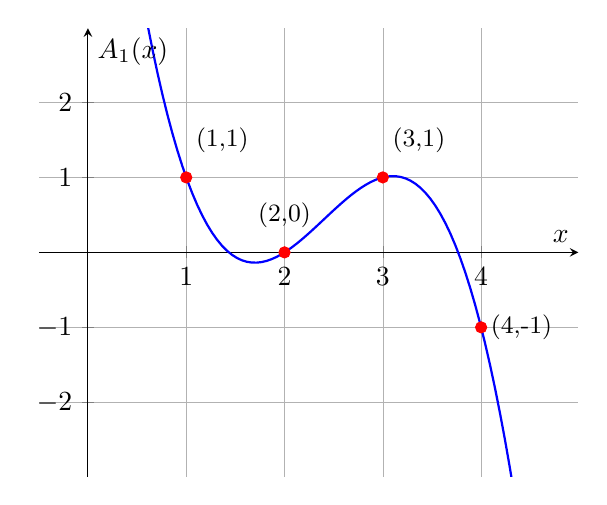
\begin{tikzpicture}
        \begin{axis}[
            axis lines = middle,
            xlabel = {$x$},
            ylabel = {$A_1(x)$},
            ymin = -2.99, ymax = 2.99,
            xmin = -0.5, xmax = 4.99,
            domain = 0:5,
            samples = 100,
            ytick = {-3,...,3},
            xtick = {0,1,...,5},
            grid = both, 
            grid style = {line width=.1pt, draw=gray!20},
            major grid style = {line width=.2pt, draw=gray!60}
        ]
        \addplot[
            color=blue,
            thick
        ]
        {-5/6*x^3 + 6*x^2 - 79/6*x + 9};
        \addplot[
            only marks,
            mark=*,
            color=red
        ]
        coordinates {(1,1) (2,0) (3,1) (4,-1)};

        \node at (axis cs:1,1.5) [anchor=west] {\small (1,1)};
        \node at (axis cs:2,0.2) [anchor=south] {\small (2,0)};
        \node at (axis cs:3,1.5) [anchor=west] {\small (3,1)};
        \node at (axis cs:4,-1) [anchor=west] {\small (4,-1)};
        
        \end{axis}
    \end{tikzpicture}
    \caption{The Lagrange inteprolation polynomial for points $\{(1,1), (2,0), (3,1), (4,-1)\}$}
    \label{fig:example-interpolation}
\end{figure}

The degree of coefficient polynomials doesn't exceed $m - 1$.

Now, using coefficients encoded with polynomials, a constraint number $X \in \{1, \dots\ m\}$, from
a constraint system with a witness vector $\mathbf{w}$ can be built in the next way:
\begin{align*}
    (w_1A_1(X) + w_2A_2(X) + \dots + w_nA_n(X)) &\times (w_1B_1(X) + w_2B_2(X) + \dots + w_nB_n(X)) =\\ = (w_1C_1(X) + w_2C_2(X)& + \dots + w_nC_n(X))
\end{align*}
Or:
\begin{align*}
    \left( \sum_{i = 1}^{n} w_iA_i(X) \right) \times \left( \sum_{i = 1}^{n} w_iB_i(X) \right) = \left( \sum_{i = 1}^{n} w_iC_i(X) \right)
\end{align*}

\begin{remark}
    Some pretty obvious property should be noted. In the theorem ~\ref{thm:polynomials-degree-op}
    it was said about the degree of polynomials after their multiplication or addition, but what
    about their values?

    Let $p(x), q(x) \in \mathbb{F}[x]$ be two polynomials over a field $\mathbb{F}$. Define the 
    polynomial $r(x)$ as the sum of $p(x)$ and $q(x)$:
    \begin{equation*}
        r(x) = p(x) + q(x)
    \end{equation*}
    Then, for any point $x \in \mathbb{F}$, the value of $r(x)$ is equal to the sum of the
    values of $p(x)$ and $q(x)$ at that point. Therefore, the set of points corresponding to the 
    polynomial $r(x)$ is given by:
    \begin{equation*}
        \{(x, y) \in \mathbb{F} \times \mathbb{F} \mid x \in \mathbb{F}, \, y = p(x) + q(x) \}
    \end{equation*}

    The same is true for product.
\end{remark}

\begin{example}
    Consider two polynomials $p(x)$ and $q(x)$ defined over the real numbers $\mathbb{R}$:
    \begin{equation*}
        p(x) = -\frac{1}{2}x^2 + \frac{3}{2}x, \quad
        q(x) = \frac{1}{3}x^3 - 2x^2 + \frac{8}{3}x + 1.
    \end{equation*}
    The sets of points $\{(0, 0), (1, 1), (2, 1), (3, 0)\}$ and $\{(0, 1), (1, 2), (2, 1), (3, 0)\}$
    lie on the graphs of $p(x)$ and $q(x)$, respectively.\\
    
    The sum of these polynomials can be calculated as:
    \begin{align*}
        r(x) &= (-\frac{1}{2}x^2 + \frac{3}{2}x) + (\frac{1}{3}x^3 - 2x^2 + \frac{8}{3}x + 1) \\
             &= \frac{1}{3}x^3 - 2\frac{1}{2}x^2 + 4\frac{1}{6}x + 1
    \end{align*}
    The resulting polynomial $r(x)$ corresponds to the set of points $\{(0, 1), (1, 3), (2, 2), (3, 0)\}$.
    
    As you can see (Figure~\ref{fig:example-polynomial-addition}), the values at each point for the 
    corresponding $x$ are the sum of the initial polynomials' points.
\end{example}

\begin{figure}[H]
    \centering
    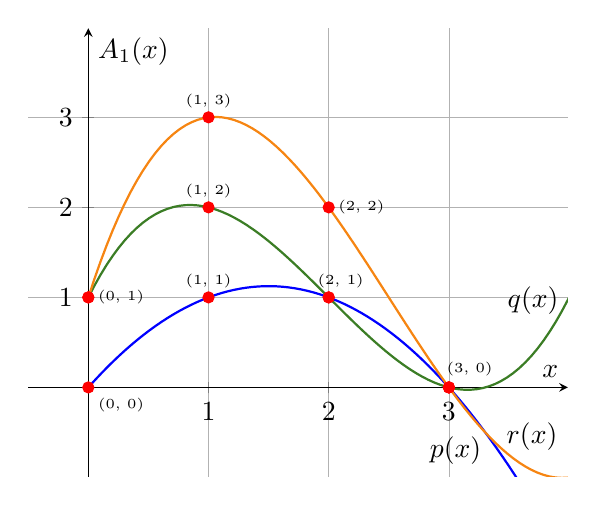
\begin{tikzpicture}
        \begin{axis}[
            axis lines = middle,
            xlabel = {$x$},
            ylabel = {$A_1(x)$},
            ymin = -0.99, ymax = 3.99,
            xmin = -0.5, xmax = 3.99,
            domain = 0:5,
            samples = 100,
            ytick = {-1,...,4},
            xtick = {0,1,...,4},
            grid = both,
            grid style = {line width=.1pt, draw=gray!20},
            major grid style = {line width=.2pt, draw=gray!60}
        ]

        % p(x)
        \addplot[
            color=blue,
            thick
        ]
        {3/2*x - 1/2*x^2};
        \addplot[
            only marks,
            mark=*,
            color=red
        ]
        coordinates {(0, 0) (1, 1) (2, 1) (3, 0)};
        \node at (axis cs:3.35,-0.7) [anchor=east] {\text{$p(x)$}};

        \node at (axis cs:0,-0.2) [anchor=west] {\tiny (0, 0)};
        \node at (axis cs:1,1) [anchor=south] {\tiny (1, 1)};
        \node at (axis cs:2.1,1) [anchor=south] {\tiny (2, 1)};
        \node at (axis cs:2.9,0.2) [anchor=west] {\tiny (3, 0)};

        % q(x)
        \addplot[
            color=OliveGreen,
            thick
        ]
        {1/3*x^3 - 2*x^2 + 8/3*x + 1};
        \addplot[
            only marks,
            mark=*,
            color=red
        ]
        coordinates {(0,1) (1,2) (2,1) (3, 0)};
        \node at (axis cs:3.7,0.7) [anchor=south] {\text{$q(x)$}};

        \node at (axis cs:0,1) [anchor=west] {\tiny (0, 1)};
        \node at (axis cs:1,2) [anchor=south] {\tiny (1, 2)};

        % r(x)
        \addplot[
            color=BurntOrange,
            thick
        ]
        {1/3*x^3 - 5/2*x^2 + 25/6*x + 1};
        \addplot[
            only marks,
            mark=*,
            color=red
        ]
        coordinates {(0,1) (1,3) (2,2) (3, 0)};
        \node at (axis cs:3.4,-0.55) [anchor=west] {\text{$r(x)$}};

        \node at (axis cs:1,3) [anchor=south] {\tiny (1, 3)};
        \node at (axis cs:2,2) [anchor=west] {\tiny (2, 2)};

        \end{axis}
    \end{tikzpicture}
    \caption{Addition of two polynomials}
    \label{fig:example-polynomial-addition}
\end{figure}

\end{document}